% $Header: /cvsroot/latex-beamer/latex-beamer/solutions/conference-talks/conference-ornate-20min.en.tex,v 1.6 2004/10/07 20:53:08 tantau Exp $

\documentclass[trans,aspectratio=1610]{beamer}
\usepackage{etex}
\newcommand\orh{\mbox{ ; }}
% This file is a solution template for:
\usepackage{amsmath}
\usepackage{amsthm,amssymb,mathabx,amsbsy}
\usepackage{xspace}
\usepackage[all]{xy}
% - Talk at a conference/colloquium.
% - Talk length is about 20min.
% - Style is ornate.
\DeclareMathOperator*{\argmax}{arg\,max}
\DeclareMathOperator*{\argmin}{arg\,min}
\newcommand{\defprog}{\ensuremath{P}\xspace}
\newcommand{\lpnot}[1][\!\!]{\sim#1}
\newcommand{\defpprog}{\ensuremath{\mathcal{P}}\xspace}
\newcommand{\lpif}{\leftarrow}

% Copyright 2004 by Till Tantau <tantau@users.sourceforge.net>.
%
% In principle, this file can be redistributed and/or modified under
% the terms of the GNU Public License, version 2.
%
% However, this file is supposed to be a template to be modified
% for your own needs. For this reason, if you use this file as a
% template and not specifically distribute it as part of a another
% package/program, I grant the extra permission to freely copy and
% modify this file as you see fit and even to delete this copyright
% notice.
%\usepackage{xcolor}
\usepackage{graphicx}
\usepackage{array}
\usepackage[all]{xy}
%\usepackage{theapa}
\usepackage{tikz}
\usetikzlibrary{snakes,arrows,shapes,arrows.meta}

\usetikzlibrary{shapes.geometric}
\usetikzlibrary{shadows}
\usetikzlibrary{positioning}
\usepackage{algorithm}
%\usepackage{algorithmic}
\usepackage{algpseudocode}
\usepackage{natbib}

\usepackage{apalike}
\mode<presentation>
{
%  \usetheme{AnnArbor}
%  \usetheme{Antibes}
%  \usetheme{Bergen}
%  \usetheme{Berkeley}
%  \usetheme{Berlin}
%  \usetheme{Boadilla}
%  \usetheme{boxes}
%  \usetheme{CambridgeUS}
%  \usetheme{Copenhagen}
%  \usetheme{Darmstadt}
%  \usetheme{default}
%  \usetheme{Dresden}
%  \usetheme{Frankfurt}
%  \usetheme{Goettingen}
%  \usetheme{Hannover}
%  \usetheme{Ilmenau}
%  \usetheme{JuanLesPins}
%  \usetheme{Luebeck}
%  \usetheme{Madrid}
%  \usetheme{Malmoe}
%  \usetheme{Marburg}
%  \usetheme{Montpellier}
%  \usetheme{PaloAlto}
%  \usetheme{Pittsburgh}
%  \usetheme{Rochester}
%  \usetheme{Singapore}
%  \usetheme{Szeged}
%  \usetheme{Warsaw}
  \usetheme{PLP}
  
%\usecolortheme{lily}%
  % or ...

  \setbeamercovered{transparent}
  % or whatever (possibly just delete it)
}

\newcommand\cA{{\cal A}}
\newcommand\cB{{\cal B}}
\newcommand\cC{{\cal C}}
\newcommand\cD{{\cal D}}
\newcommand\cE{{\cal E}}
\newcommand\cF{{\cal F}}
\newcommand\cG{{\cal G}}
\newcommand\cH{{\cal H}}
\newcommand\cI{{\cal I}}
\newcommand\cJ{{\cal J}}
\newcommand\cK{{\cal K}}
\newcommand\cL{{\cal L}}
\newcommand\cN{{\cal N}}
\newcommand\cP{{\cal P}}
\newcommand\cR{{\cal R}}
\newcommand\cS{{\cal S}}
\newcommand\cT{{\cal T}}
\newcommand\cU{{\cal U}}
\newcommand\cV{{\cal V}}
\newcommand\cW{{\cal W}}
\newcommand\cX{{\cal X}}
\newcommand\cM{{\cal M}}
\newcommand\f{\litF}
\newcommand\WMC{\mathit{WMC}}
\newcommand{\pair}[2]{\ensuremath{\langle {#1}, {#2}\rangle}}
\newcommand{\vecranvar}[1]{%
\ensuremath{\mathbf{\ranvar{#1}}}}
\newcommand{\ranvar}[1]{%
\ensuremath{{#1}}}
\newcommand{\fp}{\mathit{fp}}
\newcommand{\tp}{\mathit{tp}}
\newcommand{\TP}{\mathit{TP}}
\newcommand{\FP}{\mathit{FP}}
\newcommand{\TN}{\mathit{TN}}
\newcommand{\FN}{\mathit{FN}}



\usepackage[english]{babel}
% or whatever

%\usepackage[latin1]{inputenc}
% or whatever

\usepackage{times}
\usepackage[T1]{fontenc}
% Or whatever. Note that the encoding and the font should match. If T1
% does not look nice, try deleting the line with the fontenc.
\newcommand{\myalert}[1]{{%\color{red}
 #1}}
\newcommand{\fluffy}{\mathit{fluffy}}
\newcommand{\bdd}[2]
{
\begin{center}
\begin{tikzpicture}
[every node/.style={font=\scriptsize,minimum height=0.5cm,minimum width=0.5cm},x=2cm,y=1.2cm,rounded corners=2mm,zeroarrow/.style = {-stealth,dashed},
  onearrow/.style = {-stealth,solid},
  c/.style = {circle,draw,solid,minimum width=2em,
        minimum height=2em},
  r/.style = {rectangle,draw,solid,minimum width=2em,
        minimum height=2em}]
%[place/.style={shape=ellipse}]
%,draw=blue!50,fill=blue!20,thick,inner sep=0pt,minimum size=6mm},

\node[c] (X11) at (0,1) {#1};
   \node[c] (X21) at (1,1.5) {#2};
   \node[r] (final-one) at (2,0.5) {1};
   \node[r] (final-zero) at (2,1.5){0};
\node[] (lX11) at (0,0) {#1};
   \node (lX21) at (1,0) {#2};


   \path[onearrow,bend right=20] (X11) edge (final-one) ;
   \path[onearrow,bend right=20] (X21) edge   (final-one) ;

%      \draw[onearrow] (X11) -- (final-one);
%   \draw[onearrow] (X21) -- (final-one);

   \path[zeroarrow,bend left=20] (X11) edge  (X21) ;
   \path[zeroarrow,bend left=20] (X21) edge  (final-zero) ;
%
%   \draw[zeroarrow] (X11) -- (X21);
%   \draw[zeroarrow] (X21) -- (final-zero);
%
%\node (root) at ( 0,1) {};
%\node (node21) at ( 1,1.5){}  ;
%\node (0) at ( 2,1.5) {0};
%\node (1) at ( 2,0.5) {1};
%\path[-,bend left](node21) edge (0) (root) edge node {0} (node21);
%\path[-,bend right]
%			 (root) edge (1)
%(node21) edge (1);
\end{tikzpicture}
\end{center}
}


\newcommand{\mdd}
{
\begin{center}
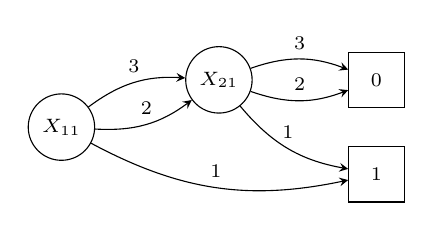
\begin{tikzpicture}
[every node/.style={font=\scriptsize},x=2cm,y=1.2cm,
zeroarrow/.style = {-stealth,dashed},
  onearrow/.style = {-stealth,solid},
  c/.style = {circle,draw,solid,minimum width=2em,
        minimum height=2em},
  r/.style = {rectangle,draw,solid,minimum width=2em,
        minimum height=2em}]
%[place/.style={shape=ellipse}]
%,draw=blue!50,fill=blue!20,thick,inner sep=0pt,minimum size=6mm},

\node[c] (X11) at (0,1) {$X_{11}$};
   \node[c] (X21) at (1,1.5) {$X_{21}$};
   \node[r] (final-one) at (2,0.5) {1};
   \node[r] (final-zero) at (2,1.5){0};

   \path[onearrow,bend right=20] (X11) edge   node [above,midway] {1}(final-one) ;
   \path[onearrow,bend right=20] (X21) edge   node [above,midway] {1}(final-one) ;

   \path[onearrow,bend right=20] (X11) edge   node [above,midway] {2}(X21) ;
   \path[onearrow,bend left=20] (X11) edge   node [above,midway] {3}(X21) ;
   \path[onearrow,bend right=20] (X21) edge   node [above,midway] {2}(final-zero) ;
   \path[onearrow,bend left=20] (X21) edge   node [above,midway] {3}(final-zero) ;
%
%\node (root) at ( 0,1) {};
%\node (node21) at ( 1,1.5){}  ;
%\node (0) at ( 2,1.5) {0};
%\node (1) at ( 2,0.5) {1};
%\path[-,bend left](node21) edge (0) (root) edge node {0} (node21);
%\path[-,bend right]
%			 (root) edge (1)
%(node21) edge (1);
\end{tikzpicture}
\end{center}
}
\newcommand{\mn}{
\begin{center}
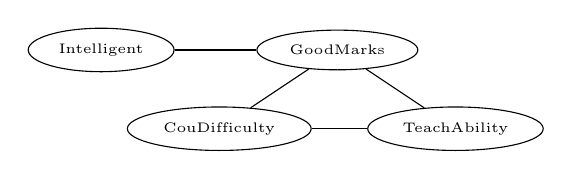
\begin{tikzpicture}
[every node/.style={ellipse,draw,font=\tiny},x=1.5cm,y=1cm]
%[place/.style={shape=ellipse}]
%,draw=blue!50,fill=blue!20,thick,inner sep=0pt,minimum size=6mm},
\node (VisitToAsia) at ( 0,1) {Intelligent};
\node (Tubercolosis) at ( 2,1) [ellipse,draw] {GoodMarks};
\node (Asthma) at ( 1,0) [ellipse,draw] {CouDifficulty};
\node (Cough) at ( 3,0) [ellipse,draw] {TeachAbility};
\path (VisitToAsia) edge  (Tubercolosis)
			 (Tubercolosis) edge (Asthma) edge (Cough)
			(Asthma) edge (Cough);
\end{tikzpicture}\end{center}}

\newcommand{\mln}{
\begin{center}
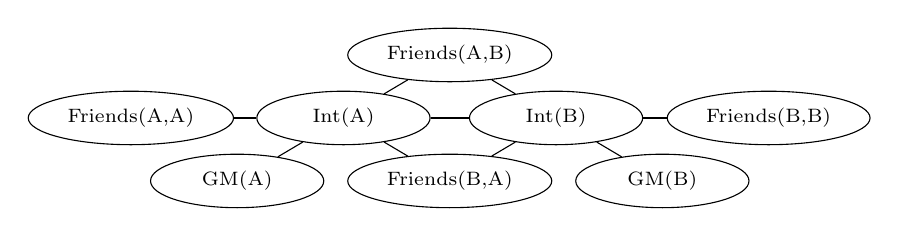
\begin{tikzpicture}
%[every node/.style={ellipse,draw,font=\scriptsize,minimum height=0.5cm,minimum width=2.5cm,
[every node/.style={ellipse,draw,font=\scriptsize,minimum width=2.2cm},x=2.7cm,y=0.8cm]

%[place/.style={shape=ellipse}]
%,draw=blue!50,fill=blue!20,thick,inner sep=0pt,minimum size=6mm},
\node (FriendsAB) at ( 1.5,2) {Friends(A,B)};
\node (FriendsAA) at ( 0,1)  {Friends(A,A)};
\node (FriendsBB) at ( 3,1)  {Friends(B,B)};
\node (FriendsBA) at ( 1.5,0)  {Friends(B,A)};
\node (SmokesA) at ( 1,1)  {Int(A)};
\node (SmokesB) at ( 2,1)  {Int(B)};
\node (CancerA) at ( 0.5,0)  {GM(A)};
\node (CancerB) at ( 2.5,0)  {GM(B)};
\path (FriendsAA) edge  (SmokesA)
		(CancerA) edge (SmokesA)
	(FriendsBB) edge  (SmokesB)
		(CancerB) edge (SmokesB)
	(FriendsAB) edge  (SmokesA)
					edge  (SmokesB)
	(FriendsBA) edge  (SmokesA)
					edge  (SmokesB)
			(SmokesB) edge (SmokesA);

%			 (Tubercolosis) edge (Asthma) edge (Cough)
%			(Asthma) edge (Cough);
\end{tikzpicture}
\end{center}
}


\newcommand{\bn}{
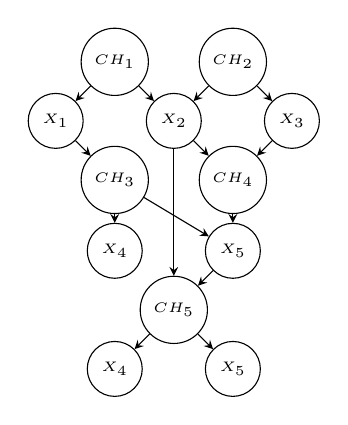
\begin{tikzpicture}
[every node/.style={draw,font=\tiny},x=0.75cm,y=0.75cm,rounded corners=2mm,zeroarrow/.style = {-stealth,dashed},
  onearrow/.style = {-stealth,solid},
  c/.style = {circle,draw,solid},
  r/.style = {rectangle,draw,solid,minimum width=1em,
        minimum height=1em}]
%[place/.style={shape=ellipse}]
%,draw=blue!50,fill=blue!20,thick,inner sep=0pt,minimum size=6mm},

\node[c] (CH1) at (1,5) {$CH_1$};
\node[c] (CH2) at (3,5) {$CH_2$};
\node[c] (X1) at (0,4) {$X_1$};
\node[c] (X2) at (2,4) {$X_2$};
\node[c] (X3) at (4,4) {$X_3$};
\node[c] (CH3) at (1,3) {$CH_3$};
\node[c] (CH4) at (3,3) {$CH_4$};
\node[c] (X4) at (1,1.8) {$X_4$};
\node[c] (X5) at (3,1.8) {$X_5$};
\node[c] (CH5) at (2,0.8) {$CH_5$};
\node[c] (X6) at (1,-0.2) {$X_4$};
\node[c] (X7) at (3,-0.2) {$X_5$};
%
%   \node[c] (X21) at (1,1.5) {#2};
%   \node[r] (final-one) at (2,0.5) {1};
%   \node[r] (final-zero) at (2,1.5){0};
%
%
   \path[onearrow] (CH1) edge (X1) ;
   \path[onearrow] (CH1) edge (X2) ;
   \path[onearrow] (CH2) edge (X2) ;
   \path[onearrow] (CH2) edge (X3) ;
   \path[onearrow] (X1) edge (CH3) ;
   \path[onearrow] (X2) edge (CH4) ;
   \path[onearrow] (X3) edge (CH4) ;
   \path[onearrow] (CH3) edge (X4) ;
   \path[onearrow] (CH3) edge (X5) ;
   \path[onearrow] (CH4) edge (X5) ;
   \path[onearrow] (X2) edge (CH5) ;
   \path[onearrow] (X5) edge (CH5) ;
   \path[onearrow] (CH5) edge (X6) ;
   \path[onearrow] (CH5) edge (X7) ;

%
%%      \draw[onearrow] (X11) -- (final-one);
%%   \draw[onearrow] (X21) -- (final-one);
%
%   \path[zeroarrow,bend left=20] (X11) edge  (X21) ;
%   \path[zeroarrow,bend left=20] (X21) edge  (final-zero) ;
%
%   \draw[zeroarrow] (X11) -- (X21);
%   \draw[zeroarrow] (X21) -- (final-zero);
%
%\node (root) at ( 0,1) {};
%\node (node21) at ( 1,1.5){}  ;
%\node (0) at ( 2,1.5) {0};
%\node (1) at ( 2,0.5) {1};
%\path[-,bend left](node21) edge (0) (root) edge node {0} (node21);
%\path[-,bend right]
%			 (root) edge (1)
%(node21) edge (1);
\end{tikzpicture}
}
%\addtobeamertemplate{background canvas}{\transuncover}{}

\title[PLP - Ch 9]
{Foundations of Probabilistic Logic Programming}
\subtitle{Chapter 9: Parameter Learning}
%\subtitle{Week 1, lecture 1: syntax, semantics and exact inference}


\author[F. Riguzzi] % (optional, use only with lots of authors)
{Fabrizio Riguzzi}
% - Give the names in the same order as the appear in the paper.
% - Use the \inst{?} command only if the authors have different
%   affiliation.

\institute[] % (optional, but mostly needed)
{
}
% - Use the \inst command only if there are several affiliations.
% - Keep it simple, no one is interested in your street address.


\subject{PILP}
% This is only inserted into the PDF information catalog. Can be left
% out.



% If you have a file called "university-logo-filename.xxx", where xxx
% is a graphic format that can be processed by latex or pdflatex,
% resp., then you can add a logo as follows:
%\logo{\includegraphics[scale=0.12]{LogoUnife}}
\date{}


% Delete this, if you do not want the table of contents to pop up at


% If you wish to uncover everything in a step-wise fashion, uncomment
% the following command:

%\beamerdefaultoverlayspecification{<+->}
%\AtBeginSection[]
%{
%\begin{frame}
%\frametitle{Outline}
%\end{frame}
%}
\begin{document}
\begin{frame}
\titlepage
\vspace{-2cm}
\begin{center}

\includegraphics[scale=0.120]{plp-book.jpg}


\includegraphics[scale=0.3]{cc-by.png}

\end{center}
\end{frame}



\begin{frame}
  \frametitle{Outline}

\begin{itemize}
\item PRISM
\item EMBLEM
\item LeProbLog
\item LFI-Problog
\end{itemize}
\end{frame}

\begin{frame}
  \frametitle{PRISM}
\begin{definition}[PRISM parameter learning problem]
\index{PRISM!learning task}
Given a PRISM program \defpprog and a set of examples $E=\{e_1,\ldots,e_T\}$ which
are ground atoms,
find the parameters of $msw$ fact so that the \emph{likelihood} of the  atoms 
$$L=\prod_{t=1}^T P(e_t)$$
 is 
maximized.

Equivalently, find the parameters of $msw$ fact so that the log likelihood of the  atoms 
$$LL=\sum_{t=1}^T \log P(e_t)$$ is maximized.
\end{definition}
\end{frame}
\begin{frame}
  \frametitle{PRISM Assumpions}
\begin{enumerate}
\item  the probability of a conjunction
$(A, B)$ is computed as the product of the probabilities of $A$ and $B$ (\emph{independent-and assumption}), \label{ind}\index{independent-and assumption}
\item
the probability of a disjunction $(A; B)$ is computed as the sum of the probabilities of $A$ and $B$
(\emph{exclusive-or assumption}). \label{ex}\index{exclusive-or assumption}
\end{enumerate}
  \end{frame}
\begin{frame}
  \frametitle{Example}
  \begin{itemize}
\item Hidden Markov model:  a dynamical system that,
at each  time point $t$,  is in a state $S$ and
emits  one symbol $O$ 
\item  $P(O|S)$  and
$P(NextS|S)$ are independent of time.
\item The states are  hidden:
the task is to obtain information on them from the sequence of output symbols.
\item Speech recognition.
\end{itemize}
\end{frame}
\begin{frame}
  \frametitle{Example}

$\begin{array}{l}
values(tr(s1),[s1,s2]).\\
values(tr(s2),[s1,s2]).\\
values(out(\_),[a,b]).\\
hmm(Os)\lpif hmm(s1,Os).\\
hmm(\_S,[]).\\ 
hmm(S,[O|Os])\lpif \\
\ \ \ \ 
  msw(out(S),O),  msw(tr(S),NextS),  
  hmm(Next,Os).
\end{array}$

  \begin{itemize}
\item  $P(hmm(Os))$:
probability that the sequence of symbols $Os$ is emitted.
\item No \alert{memoing}.
\end{itemize}
\end{frame}



\begin{frame}
  \frametitle{Example}
  \begin{itemize}
\item Query $hmm([a,b,b])$ 
\item 8 explanations
\end{itemize}
$\begin{array}{l}
E_1=m(out(s1),a),m(tr(s1),s1),m(out(s1),b),m(tr(s1),s1),\\
\ \ \ \ m(out(s1),b),m(tr(s1),s1),\\
E_2=m(out(s1),a),m(tr(s1),s1),m(out(s1),b),m(tr(s1),s1),\\
\ \ \ \ m(out(s1),b),m(tr(s1),s2),\\
E_3=m(out(s1),a),m(tr(s1),s1),m(out(s2),b),m(tr(s1),s2),\\
\ \ \ \ m(out(s2),b),m(tr(s2),s1),\\
\ldots\\
E_8=m(out(s1),a),m(tr(s1),s2),m(out(s2),b),m(tr(s2),s2),\\
\ \ \ \ m(out(s2),b),m(tr(s2),s2)\\
\end{array}$
\end{frame}
\begin{frame}
  \frametitle{Example}
 \begin{itemize}
\item If the query $q$ has the explanations $E_1\ldots,E_n$:
$$q\Leftrightarrow E_1\vee\ldots\vee E_n$$
\item  $P(q)=\sum_{i=1}^n P(E_i)$
\item  $P(E_i)$ is the product of the probability of each atom
\item Because of the assumptions
\end{itemize}
\end{frame}



\begin{frame}[fragile]
  \frametitle{PRISM}
\begin{verbatim}
values(gene,[a,b,o]).
bloodtype(P) :-
  genotype(X,Y),
  ( X=Y -> P=X
  ; X=o -> P=Y
  ; Y=o -> P=X
  ; P=ab
  ).
genotype(X,Y) :- msw(gene,X),msw(gene,Y).
\end{verbatim}
How a person's blood type is determined by his genotype, formed by a pair of two genes (\verb|a|, \verb|b|
or \verb|o|).
\end{frame}
\begin{frame}[fragile]
  \frametitle{PRISM}
  \begin{scriptsize}
\begin{verbatim}
?- learn([count(bloodtype(a),40),count(bloodtype(b),20),
    count(bloodtype(o),30),count(bloodtype(ab),10)]).
\end{verbatim}
\end{scriptsize}
where \verb|count(At,N)| denotes the repetition of atom \verb|At| \verb|N| times.
\begin{scriptsize}
\begin{verbatim}
?- show_sw.
Switch gene: unfixed: a (0.292329558535712) 
b (0.163020241540856)
o (0.544650199923432)
\end{verbatim}
\end{scriptsize}
\end{frame}
\begin{frame}
  \frametitle{PRISM}
\begin{itemize}
\item
 PRISM looks for the maximum likelihood parameters\index{maximum likelihood} of the $msw$ atoms. 
 \item These are
not observed in the dataset, which contains only derived atoms. 
\item Relative frequency
\index{relative frequency}
cannot be used 
\item Expectation Maximization
\end{itemize}
\end{frame}
\begin{frame}
  \frametitle{PRISM}
\begin{itemize}
\item Associate a random variable $X_{ij}$ with values $D=\{x_{i1},\ldots,x_{in_i}\}$ to the ground switch name $i\theta_j$  of $msw(i,x)$ with domain $D$, with $\theta_j$ being a grounding
substitution for $i$. 
$$g(i)=\{j|\theta_j \mbox{ is a grounding substitution for $i$ in } msw(i,x) \}.$$
\item PRISM alternates between the two phases:
\begin{itemize}
\item 
Expectation:
computes $\mathbf{E}[c_{ijk}|e]$ for all examples $e$, switches $msw(i\theta_j,x)$ and $k\in\{1,\ldots,n_i\}$, where $c_{ijk}$ is the number of times  variable $X_{ij}$ takes value $x_{ik}$
$$\mathbf{E}[c_{ijk}|e]=P(X_{ij}=x_{ik}|e).$$
\item
Maximization: computes $\Pi_{ijk}$ for all $msw(i\theta_j,x)$ and $k=1,\ldots,n_i-1$ as
$$\Pi_{ijk}=\frac{\sum_{e\in E}\mathbf{E}[c_{ijk}|e]}{\sum_{e\in E}\sum_{k=1}^{n_i}\mathbf{E}[c_{ijk}|e]}$$
%$$\Pi_{ik}=\frac{\sum_{X_{ijk}\in i(C_{ik})}P(X_{ijk}=1|Q)}{\sum_{X_{ijk}\in i(C_i)}(P(X_{ijk}=0|Q)+P(X_{ijk}=1|Q))}$$
\end{itemize}
\end{itemize}
\end{frame}
\begin{frame}
  \frametitle{PRISM}
\begin{itemize}
\item
If the program satisfies the exclusive-or
assumption, $P(X_{ij}=x_{ik}|e)$ can be computed as
$$P(X_{ij}=x_{ik}|e)=\frac{P(X_{ij}=x_{ik},e)}{P(e)}=
\frac{\sum_{\kappa\in K_e,msw(i\theta_j,x_{ik})\in e}P(\kappa)}{P(e)}$$
where $K_e$ is the set of explanations of $e$ 
\item Each explanation $\kappa$ is a set of 
$msw$ atoms of the form $msw(i\theta_j,x_{ik})$.
\end{itemize}
\end{frame}
\begin{frame}
  \frametitle{Naive PRISM}
\begin{algorithmic}[1]
\Function{PRISM-EM-Naive}{$E,\defpprog,\epsilon$}
\State $LL=-\mathit{inf}$
\Repeat
  \State $LL_0=LL$
  \ForAll{$i,j,k$}\Comment{Expectation step}
    \State $\mathbf{E}[c_{ijk}]\gets \sum_{e\in E}\frac{\sum_{\kappa\in K_e,msw(i\theta_j,x_{ik})\in e}P(\kappa)}{P(e)}$
  \EndFor
  \ForAll{$i,j,k$}\Comment{Maximization step}
    \State $\Pi_{ijk}\gets \frac{ \mathbf{E}[c_{ijk}]}{\sum_{k'=1}^{n_i}\mathbf{E}[c_{ijk'}]}$
  \EndFor
  \State $LL\gets \sum_{e\in E}\log P(e)$
\Until{$LL-LL_0 < \epsilon $}
\State return $LL,\Pi_{ijk}$ for all $i,j,k$
\EndFunction
\end{algorithmic}

\end{frame}
\begin{frame}
  \frametitle{PRISM}
  \begin{itemize}
\item There can be  exponential numbers of explanations
\item More efficient dynamic programming algorithm
\item
Tabling is used to find formulas of the form
$$g_{i}\Leftrightarrow S_{i1}\vee\ldots\vee S_{is_i}$$
\item The $g_i$s are  subgoals  that can be ordered as
$\{g_1,\ldots,g_m\}$ such that $e=g_1$ and
 each $S_{ij}$ contains only $msw$ atoms and subgoals from $\{g_{i+1},\ldots,g_{m}\}$.
\item
Linear number of  formulas  rather than exponential
\item  \alert{Acyclic support condition}, true if tabling succeeds in 
evaluating $q$, i.e., if it doesn't go into a loop.
\end{itemize}
\end{frame}

\begin{frame}
  \frametitle{Example}
  \begin{itemize}
\item For
$hmm([a,b,b])$, PRISM builds
the formulas 
\end{itemize}
\begin{scriptsize}
$\begin{array}{l}
hmm([a,b,b])\Leftrightarrow hmm(s1,[a,b,b])\\
hmm(s1,[a,b,b]) \Leftrightarrow m(out(s1),a),m(tr(s1),s1),hmm(s1,[b,b])\vee\\
\ \ \ \ m(out(s1),a),m(tr(s1),s2),hmm(s2,[b,b])\\
hmm(s1,[b,b]) \Leftrightarrow m(out(s1),b),m(tr(s1),s1),hmm(s1,[b])
\vee\\
\ \ \ \ m(out(s1),b),m(tr(s1),s2),hmm(s2,[b])\\
hmm(s2,[b,b]) \Leftrightarrow m(out(s2),b),m(tr(s2),s1),hmm(s1,[b])
\vee\\
\ \ \ \ m(out(s2),b),m(tr(s2),s2),hmm(s2,[b])\\
hmm(s1,[b]) \Leftrightarrow m(out(s1),b),m(tr(s1),s1),hmm(s1,[])\vee\\
\ \ \ \  m(out(s1),b),m(tr(s1),s2),hmm(s2,[])\\
hmm(s2,[b]) \Leftrightarrow m(out(s2),b),m(tr(s2),s1),hmm(s1,[])\vee\\
\ \ \ \  m(out(s2),b),m(tr(s2),s2),hmm(s2,[])\\
hmm(s1,[]) \Leftrightarrow true\\
hmm(s2,[]) \Leftrightarrow true
\end{array}$
\end{scriptsize}
\end{frame}

\begin{frame}
  \frametitle{PRISM}
  \begin{itemize}
  \item PRISM  computes, for each example, the probability
$P(g_i)$ 
of the subgoals $\{g_1,\ldots,g_m\}$, also called the \emph{inside probability}, 
\item and the value $Q(g_i)$ which is 
called the
\emph{outside probability}. 
\item  PRISM  generalizes the Inside-Outside algorithm
\index{Inside-Outside algorithm} for PCFG.
\item  It also generalizes the forward-backward 
\index{forward-backward} algorithm  for parameter 
learning in HMM by the Baum-Welch algorithm
\end{itemize}
\end{frame}
\begin{frame}
  \frametitle{Get-Inside-Probs}
\begin{algorithmic}[1]
\Procedure{Get-Inside-Probs}{$q$}
\ForAll{$i,j,k$}
  \State $P(msw(i\theta_j,v_k))\gets \Pi_{ijk}$
\EndFor
\For{$i\gets m \to 1$}
  \State   $P(g_i)\gets 0$
  \For{$j\gets 1 \to s_i$}
    \State Let $S_{ij}$ be $h_{ij1},\ldots,h_{ijo}$
    \State $P(g_i,S_{ij})\gets\prod_{l=1}^{o}P(h_{ijl})$
    \State   $P(g_i)\gets P(g_i)+P(g_i,S_{ij})$  
  \EndFor
\EndFor
\EndProcedure
\end{algorithmic}
\end{frame}
\begin{frame}
  \frametitle{Outside probabilities}
  \begin{itemize}
  \item 
Defined as
$$Q(g_i)=\frac{\partial P(q)}{\partial P(g_i)}$$
\item 
Suppose $g_i$ appears in the  ground program as
$$\begin{array}{ccc}
b_1\lpif g_i, W_{11}& \ldots& b_1\lpif g_i, W_{1i_1}\\
&\ldots&\\
b_K\lpif g_i, W_{K1}& \ldots& b_K\lpif g_i, W_{Ki_K}\\
\end{array}$$
\item Then
$$\begin{array}{c}
P(b_1)=P( g_i, W_{11})+ \ldots+ P(g_i, W_{1i_1})\\
\ldots\\
P(b_K)=P( g_i, W_{K1})+ \ldots+ P(g_i, W_{Ki_K})\\
\end{array}$$
\end{itemize}
\end{frame}
\begin{frame}
  \frametitle{Outside probabilities}
  \begin{itemize}
  \item $Q(g_1)=1$ as $q=g_1$. 
  \item For $i=2,\ldots,m$, 
$Q(g_i)$ by the chain rule knowing that $P(q)$ is a function 
of $P(b_1),\ldots,P(b_K)$
\begin{eqnarray*}
Q(g_i)&=&\frac{\partial P(q)}{\partial P(b_1)}\frac{\partial P(g_i,W_{11})}{\partial P(g_1)}+\ldots+
\frac{\partial P(q)}{\partial P(b_K)}\frac{\partial P(g_i,W_{Ki_K})}{\partial P(g_1)}=\\
&&Q(b_1)P(g_i,W_{11})/P(g_i)+\ldots+P(g_i,W_{Ki_K})/P(g_i)
\end{eqnarray*}
\item Recursive formula
\begin{eqnarray*}
Q(g_1)&=&1\\
Q(g_i)&=&Q(b_1)\sum_{s=1}^{i_1}\frac{P(g_i,W_{1s})}{P(g_i)}+\ldots+Q(b_K)\sum_{s=1}^{i_K}\frac{P(g_i,W_{Ks})}{P(g_i)}
\end{eqnarray*}
\item To be evaluated top-down from $q=g_1$ down to $g_m$. 
\end{itemize}
\end{frame}
\begin{frame}
  \frametitle{Outside probabilities}
  \begin{itemize}
\item We can divide the
explanations for $e$ into two sets, $K_{e1}$, that includes the explanations containing $msw(i\theta_j,x_k)$, and $K_{e2}$, that includes the other explanations.
\item   $P(e)=P(K_{e1})+ P(K_{e2})$
\item 
$P(X_{ij}=x_{ik},e)=P(K_{e1})$.
\item Each explanation in $K_{e1}$  takes the form
$\{\{g_i, W_{1}\}, \ldots,\{ g_i, W_{s}\}\}$ and
\begin{eqnarray}
P(K_{e1})&=&\sum_{\{g_i, W\} \in K_{e1}}P(g_i)P(W)=P(g_i)\sum_{\{g_i, W\} \in K_{e1}}P(W)
\end{eqnarray}
\end{itemize}
\end{frame}
\begin{frame}
  \frametitle{Outside probabilities}
  \begin{itemize}
  \item
So we obtain
\begin{eqnarray}
P(X_{ij}=x_{ik},e)&=&P(g_i)\sum_{\{g_i, W\} \in K_{e1}}P(W)=\nonumber\\
&&\frac{\partial P(K_{e})}{\partial P(g_i)}P(g_i)=\label{pen}\\
&&\frac{\partial P(e)}{\partial P(g_i)}P(g_i)=Q(g_i)P(g_i)\nonumber
\end{eqnarray}
  \item
If $g_i=msw(i\theta_j,x_k)$, then 
$$P(X_{ij}=x_{ik},e)=Q(g_i)P(g_i)=Q(g_i)\Pi_{ijk}.$$
\end{itemize}
\end{frame}

\begin{frame}
  \frametitle{Get-Outside-Probs}
\begin{algorithmic}[1]
\Procedure{Get-Outside-Probs}{$q$}
\State   $Q(g_1)\gets 1.0$
\For{$i\gets 2 \to m$}
  \State   $Q(g_i)\gets 0.0$
\EndFor
\For{$i\gets 2 \to m$}
  \State   $Q(g_i)\gets 0.0$
  \For{$j\gets 1 \to s_i$}
    \State Let $S_{ij}$ be $h_{ij1},\ldots,h_{ijo}$
    \For{$l\gets1 \to o$}
      \State $Q(h_l)\gets Q(h_l)+Q(g_i)P(g_i,S_{ij})/P(h_{ijl})$
    \EndFor
  \EndFor
\EndFor
\EndProcedure
\end{algorithmic}
\end{frame}


\begin{frame}
  \frametitle{PRISM-EM}
\begin{algorithmic}[1]
\Function{PRISM-EM}{$E,\defpprog,\epsilon$}
\State $LL=-\mathit{inf}$
\Repeat
  \State $LL_0=LL$
  \State $LL=$ \Call{Expectation}{$E$}
  \ForAll{$i,j$}
    \State $Sum\gets\sum_{k=1}^{n_i}\mathbf{E}[c_{ijk}]$
    \For{$k=1$ to $n_i$}
      \State $\Pi_{ijk}=\frac{\mathbf{E}[c_{ijk}]}{Sum}$
    \EndFor
  \EndFor
\Until{$LL-LL_0 < \epsilon $}
\State\Return  $LL,\Pi_{ijk}$ for all $i,j,k$
\EndFunction
\end{algorithmic}
\end{frame}

\begin{frame}
  \frametitle{PRISM-Expectation}
\begin{algorithmic}[1]
\Function{PRISM-Expectation}{$E$}
\State $LL=0$
%\State $F(node)=0$
\ForAll{$e\in E$}
  \State \Call{Get-Inside-Probs}{$e$}
  \State \Call{Get-Outside-Probs}{$e$}
  \ForAll{$i,j$}
    \For{$k=1$ to $n_i$}
      \State $\mathbf{E}[c_{ijk}]=\mathbf{E}[c_{ijk}]+Q(msw(i\theta_j,x_k))\Pi_{ijk}/P(e)$
%\eta^0(r,i)=\eta^0(r,i)+\eta^0(r,i)/Prob$;   $\eta^1(r,i)=\eta^1(r,i)+\eta_t^1(r,i)/Prob$
    \EndFor
  \EndFor
  \State $LL=LL+\log P(e)$
\EndFor
\State \Return $LL$
\EndFunction
\end{algorithmic}
\end{frame}

\begin{frame}
  \frametitle{Complexity}
   \begin{itemize}
  \item PRISM has the same time complexity for programs encoding HMM and PCFG as the specific parameter learning
algorithms: the Baum-Welch
algorithm  and the Inside-Outside algorithm
  \end{itemize}
  \end{frame}
  \begin{frame}
\frametitle{Parameter Learning for ProbLog and LPADs}
\begin{itemize}
\item\ [Thon et al. ECML 2008] proposed an adaptation of EM for 
CPT-L, a simplified version of LPADs
\item\ The algorithm computes the counts efficiently by repeatedly traversing the BDDs representing the explanations
\item\ [Ishihata et al. ILP 2008] independently proposed a similar algorithm 
 \item \textsc{LFI-ProbLog} [Gutamnn et al. ECML 2011]: EM for ProbLog 
 \item EMBLEM [Riguzzi \& Bellodi IDA 2013] %\citep{BelRig13-IDA-IJ}
 adapts [Ishihata et al. ILP 2008]
%\citep{Ish-ILP2008}  
to LPADs
\end{itemize}
\end{frame}

\begin{frame}
\frametitle{EMBLEM}
\begin{definition}[EMBLEM learning problem]
Given an LPAD $\mathcal{P}$ with unknown parameters and two sets $E^+=\{e_1,\ldots,e_T\}$ and  
$E^-=\{e_{T+1},\ldots,e_Q\}$
of ground atoms (positive and negative examples), find the value of the  parameters $\boldsymbol{\Pi}$ of  $\mathcal{P}$  that maximize the 
likelihood of the examples, i.e., solve
$$\argmax_{\boldsymbol{\Pi}}P(E^+,\lpnot E^-)=\argmax_{\boldsymbol{\Pi}}\prod_{t=1}^T P(e_t)\prod_{t=T+1}^Q P(\lpnot e_t).$$
 The predicates for the atoms in $E^+$ and $E^-$ 
are called \emph{target} because the objective is to be able to better predict the truth value of atoms
for them.
\end{definition}
\end{frame}

\begin{frame}
\frametitle{Parameter Learning}
\begin{itemize}
\item 
Typically, the LPAD \defpprog has two components:
 \begin{itemize}
\item  a set of rules, annotated with parameters 
\item  a set of certain ground facts, representing background knowledge
on individual cases of a specific world
\end{itemize}
\item Useful to provide information on more than one world: a background knowledge and sets of positive and negative examples for each world 
\item Description
of one world: \emph{mega-interpretation}\index{mega-interpretation} or 
\emph{mega-example}\index{mega-example|see {mega-interpretation}}
\item Positive examples encoded
as ground facts of the mega-interpretation and the negative examples as suitably annotated 
ground facts (such as $neg(a)$ for negative example $a$) 
\item The task then is maximizing the product of the likelihood of 
the examples for all mega-interpretations.
\end{itemize}
\end{frame}




\begin{frame}
  \frametitle{Example: Bongard Problems}
\begin{itemize}
\item
Introduced by the Russian
scientist M. Bongard
\item
Pictures, some positive and some negative
\item Problem: discriminate between the two classes.
\item
The pictures contain shapes with different properties, such as small, large, pointing down, \ldots\ and different relationships between them, such as inside, above, \ldots\
\end{itemize}
\begin{center}
\includegraphics[scale=0.5,draft=false]{bongard.png}
\end{center}
\end{frame}



\begin{frame}[fragile]
  \frametitle{Data}
Each mega-examle  encodes a single picture
\begin{scriptsize}
\begin{verbatim}
begin(model(2)).
pos.
triangle(o5).
config(o5,up).
square(o4).
in(o4,o5).
circle(o3).
triangle(o2).
config(o2,up).
in(o2,o3).
triangle(o1).
config(o1,up).
end(model(2)).

begin(model(3)).
neg(pos).
circle(o4).
circle(o3).
in(o3,o4).
....
\end{verbatim}
\end{scriptsize}

\end{frame}



\begin{frame}[fragile]
  \frametitle{Program}
Theory for parameter learning and background
\begin{small}
\begin{verbatim}
pos:0.5 :-
 	circle(A),
 	in(B,A).
pos:0.5 :-
 	circle(A),
 	triangle(B).
\end{verbatim}
\end{small}
The task is to tune the two parameters
\end{frame}

\begin{frame}
\frametitle{EMBLEM}
\begin{itemize}
 \item The interpretations record the truth value of ground atoms, not of the random variables
\item Unseen data: relative frequency can't be used
\item Expectation-Maximization algorithm:
\begin{itemize}
 \item Expectation step: the distribution of the unseen variables in each instance is computed given the observed data
 \item Maximization step: new parameters are computed from the distributions using relative frequency
 \item End when likelihood does not improve anymore
\end{itemize}
\end{itemize}
\end{frame}


%
%%
%\begin{frame}
%\frametitle{Parameter Learning}
%\begin{itemize}
%\item\ [Thon et al. ECML 2008] proposed an adaptation of EM for
%CPT-L, a simplified version of LPADs
%\item\ The algorithm computes the counts efficiently by repeatedly traversing the BDDs representing the explanations
%\item\ [Ishihata et al. ILP 2008] independently proposed a similar algorithm
% \item \textsc{LFI-ProbLog} [Gutamnn et al. ECML 2011]: EM for ProbLog
% \item EMBLEM [Riguzzi \& Bellodi IDA 2013] %\citep{BelRig13-IDA-IJ}
% adapts [Ishihata et al. ILP 2008]
%%\citep{Ish-ILP2008}
%to LPADs
%\end{itemize}
%\end{frame}



\begin{frame}
 \frametitle{EMBLEM}

 \begin{itemize}
 %\item \myalert{Parameter learning \citep{BelRig11-TR}}
	%\begin{itemize}
	\item EM over Bdds for probabilistic Logic programs Efficient Mining [Bellodi and Riguzzi IDA 2013]
		\item Input: an LPAD; logical interpretations (data); \textit{target} predicate(s)
		\item \myalert{All ground atoms} in the interpretations for the target predicate(s) \myalert{correspond to as many queries}
		\item \myalert{BDDs} encode the explanations \myalert{for each query} 
\item Expectations computed with two passes over the BDDs
				\end{itemize}

\end{frame}

\begin{frame}
 \frametitle{EMBLEM}
  \begin{itemize}
\item EMBLEM encodes multi-valued random variable with Boolean random variables 
\item Variable $\ranvar{X}_{ij}$ associated with  grounding $\theta_j$ of clause $C_i$
having $n$ values. 
\item Encoding using $n-1$ Boolean variables 
$\ranvar{X}_{ij1},\ldots,\ranvar{X}_{ijn-1}.$
\item
 Equation $\ranvar{X}_{ij}=k$ for $k=1,\ldots n-1$ represented by
  $$\overline{\ranvar{X}_{ij1}}\wedge\ldots \wedge \overline{\ranvar{X}_{ijk-1}}\wedge \ranvar{X}_{ijk}$$
  \item Equation $\ranvar{X}_{ij}=n$ represented by 
  $$\overline{\ranvar{X}_{ij1}}\wedge\ldots \wedge\overline{\ranvar{X}_{ijn-1}}.$$
\item Parameters:
\begin{eqnarray*}
P(\ranvar{X}_{ij1})&=&P(\ranvar{X}_{ij}=1)\\
&\ldots&\\
 P(\ranvar{X}_{ijk})&=&\frac{P(\ranvar{X}_{ij}=k)}{\prod_{l=1}^{k-1}(1-P(\ranvar{X}_{ijl}))}
 \end{eqnarray*}
 \end{itemize}
\end{frame}

\begin{frame}
 \frametitle{EMBLEM}
  \begin{itemize}
\item Let $X_{ijk}$ for $k=1,\ldots,n_i-1$ and $j\in g(i)$ be the Boolean random variables associated with grounding 
$C_i\theta_j$ of clause $C_i$ of $\defpprog$ where $n_i$ is the number of head atoms of $C_i$ and $g(i)$ is the set
of indices of grounding substitutions of $C_i$.
		\end{itemize}
\end{frame}
\begin{frame}
 \frametitle{Example}
 
$
 \begin{array}{lllllll}
C_1&=&epidemic:0.6\orh  pandemic :0.3\lpif flu(X),cold.\\
C_2&=&cold:0.7. \\
C_3&=&flu(david).\\
C_4&=&flu(robert).
 \end{array}$
\begin{itemize}
\item
Clause $C_1$: two groundings,  random variables $X_{111}$ and $X_{112}$ and the latter with $X_{121}$ and $X_{122}$.
 \item
 $C_2$:  single grounding, random variable
 $X_{211}$.
 \end{itemize}
 \begin{scriptsize}
	{
	$$
\xymatrix@=4mm
{ X_{111} & &*=<25pt,10pt>[F-:<3pt>]{n_1}
\ar@/_/@{-}[ldd] \ar@/^/@{--}[dr]\\ 
X_{121}  &&&*=<25pt,10pt>[F-:<3pt>]{n_2} 
\ar@/_/@{-}[dll]\ar@{--}[dd] 
\\
X_{211}& *=<25pt,10pt>[F-:<3pt>]{n_3}
\ar@{-}[d] \ar@/^/@{--}[drr]  && \\
&*=<25pt,10pt>[F-:<3pt>]{1} &&*=<25pt,10pt>[F-:<3pt>]{0}}
$$
}	
 \end{scriptsize}
\end{frame}
\begin{frame}
 \frametitle{EMBLEM}

  \begin{itemize}
\item 
EMBLEM alternates between the two phases:
\begin{itemize}
\item 
Expectation:
computes $\mathbf{E}[c_{ik0}|e]$ and $\mathbf{E}[c_{ik1}|e]$ for all examples $e$, rules $C_i$ in $\defpprog$ and $k=1,\ldots,n_i-1$, where $c_{ikx}$ is the number of times a variable $X_{ijk}$ takes value $x$ for $x\in \{0,1\}$, with $j$ in $g(i)$.
$\mathbf{E}[c_{ikx}|e]$ is given by $\sum_{j\in g(i)}P(X_{ijk}=x|e).$
\item
Maximization: computes $\pi_{ik}$ for all rules $C_i$ and $k=1,\ldots,n_i-1$.
$$\pi_{ik}=\frac{\sum_{e\in E}\mathbf{E}[c_{ik1}|e]}{\sum_{e\in E}\mathbf{E}[c_{ik0}|e]+\mathbf{E}[c_{ik1}|e]}$$
%$$\pi_{ik}=\frac{\sum_{X_{ijk}\in i(C_{ik})}P(X_{ijk}=1|Q)}{\sum_{X_{ijk}\in i(C_i)}(P(X_{ijk}=0|Q)+P(X_{ijk}=1|Q))}$$
\end{itemize}
\end{itemize}
\end{frame}
%If we have more than one example the contributions of each example simply sum up when computing $\mathbf{E}[c_{ijx}]$.
%
\begin{frame}
 \frametitle{EMBLEM}
 \begin{itemize}
\item 
$P(X_{ijk}=x|e)$ is given by $P(X_{ijk}=x|e)=\frac{P(X_{ijk}=x,e)}{P(e)}$.
%\begin{eqnarray*}
%P(X_{ijk}=x,q)
%&=&
%\sum_{\sigma\in E(q)}P(q,X_{ijk}=x,\sigma)\\
%&=&\sum_{\sigma\in E(q)}P(q|\sigma)P(X_{ijk}=x|\sigma)P(\sigma)\\
%&=&\sum_{\sigma\in E(q)}P(X_{ijk}=x|\sigma)P(\sigma)%\\
%%&=&\sum_{\sigma\in E(q)}P(X_{ijk}=x|\sigma)\prod_{(C_o,\theta,p)\in\sigma}\pi_{op}
%\end{eqnarray*}
%where $E(q)$ is the set of selections of worlds where  $q$ is true, $P(X_{ijk}=1|\sigma)=1$ if $(C_i,\theta_j,k)\in\sigma$ for $k=1,\ldots,n_i-1$ and 0 otherwise and $P(X_{ijk}=0|\sigma)=1$ if $(C_i,\theta_j,k')\in\sigma$ with $k<k'$,
% for $k'=1,\ldots,n_i-1$ or if $(C_i,\theta_j,n_i)\in\sigma$ if $k=n_i$ and 0 otherwise.

%Now consider a \gls{bdt} representing the example $e$, which is a \gls{bdd} where no reduction operation has been applied, i.e., a \gls{bdd} in which every node has a single parent and all the children belong to the level immediately below. \index{binary decision tree}
\item Consider a BDD for an example $e$ built by applying only the merge rule
\end{itemize}
	{
	$$
\xymatrix@=6mm
{ X_{111} & &*=<25pt,10pt>[F-:<3pt>]{n_1}
\ar@/_/@{-}[ld] \ar@/^/@{--}[dr]\\ 
X_{121}  & *=<25pt,10pt>[F-:<3pt>]{n'_2}\ar@/_/@{-}[d]  \ar@/^/@{--}[d] &&*=<25pt,10pt>[F-:<3pt>]{n_2} 
\ar@/_/@{-}[dll]\ar@{--}[d] 
\\
X_{211}& *=<25pt,10pt>[F-:<3pt>]{n_3}
\ar@{-}[d] \ar@/^/@{--}[drr]  &&*=<25pt,10pt>[F-:<3pt>]{n'_3}
\ar@/_/@{-}[d] \ar@/^/@{--}[d]  \\
&*=<25pt,10pt>[F-:<3pt>]{1} &&*=<25pt,10pt>[F-:<3pt>]{0}}
$$
}	
\end{frame}
\begin{frame}
 \frametitle{EMBLEM}
 \begin{itemize}
\item $P(e)$ is given by the sum of the probabilities of all the paths in the BDD from the root to a 1 leaf
\item 
To compute $P(X_{ijk}=x,e)$ we  need to consider only the paths passing through the
$x$-child of a node $n$ associated with variable $X_{ijk}$ so
\begin{eqnarray*}
P(X_{ijk}=x,e)
&=&\sum_{n\in N(X_{ijk})}\pi_{ikx}F(n)B(child_x(n))=\sum_{n\in N(X_{ijk})}e^x(n)
\end{eqnarray*}
 \begin{itemize}
\item 
$F(n)$ is the \emph{forward probability}, the probability mass of the paths from the root to $n$, 
\item $B(n)$ is the \emph{backward probability}, the 
\index{backward probability} probability mass of paths from $n$ to the 1 leaf.
\end{itemize}
\end{itemize}
\end{frame}
\begin{frame}
 \frametitle{EMBLEM}
 \begin{itemize}
\item
BDD obtained by also applying  the deletion rule: paths where there is no node associated with $X_{ijk}$ can also contribute to $P(X_{ijk}=x,e)$.
\item Suppose the BDD was obtained deletong node $m$ descendant of $n$ associated with variable $X_{ijk}$ 
\item Outgoing edges of $m$ both point to $child_0(n)$. 
\item The probability mass of the two paths that were merged was $e^0(n)(1-\pi_{ik})$ and $e^0(n)\pi_{ik}$ for 
\item The first quantity contributes to 
$P(X_{ijk}=0,e)$, the latter to $P(X_{ijk}=1,e)$.
\end{itemize}
\end{frame}



\begin{frame}
 \frametitle{GetForward}
 \begin{scriptsize}
\begin{algorithmic}[1]
\Procedure{GetForward}{$root$}
\State $F(root)=1$
\State $F(n)=0$ for all nodes
\For{$l=1$ to $levels$}
\Comment{$levels$ is the number of levels of the BDD rooted at $root$}
\State $Nodes(l)=\emptyset$
\EndFor
\State $Nodes(1)=\{root\}$
\For{$l=1$ to $levels$}
\ForAll{$node \in Nodes(l)$}
\State let $X_{ijk}$ be $v(node)$, the variable associated with $node$
\If{$child_0(node)$ is not terminal}
\State $F(child_0(node))=F(child_0(node))+F(node)\cdot(1-\pi_{ik}$)
\State add $child_0(node)$ to $Nodes(level(child_0(node)))$
\Comment{$level(node)$ returns the level of $node$}
\EndIf
\If{$child_1(node)$ is not terminal}
\State $F(child_1(node))=F(child_1(node))+F(node)\cdot\pi_{ik}$
\State add $child_1(node)$ to $Nodes(level(child_1(node)))$
\EndIf
\EndFor
\EndFor
\EndProcedure
\end{algorithmic}
\end{scriptsize}
\end{frame}

\begin{frame}
 \frametitle{GetBackward}
  \begin{scriptsize}
\begin{algorithmic}[1]
\Function{GetBackward}{$node$}
\If{$node$ is a terminal}
\State \Return $value(node)$
\Else
\State let $X_{ijk}$ be $v(node)$
\State $B(child_0(node))=$\Call{GetBackward}{$child_0(node)$}
\State $B(child_1(node))=$\Call{GetBackward}{$child_1(node)$}
\State $e^{0}(node)=F(node)\cdot B(child_0(node))\cdot(1-\pi_{ik})$
\State $e^{1}(node)=F(node)\cdot B(child_1(node))\cdot\pi_{ik}$
\State $\eta^{0}(i,k)=\eta_t^{0}(i,k)+e^{0}(node)$
\State $\eta^{1}(i,k)=\eta_t^{1}(i,k)+e^{1}(node)$
%\State $VSucc=succ(v(node))$\Comment{$succ(X)$ returns the variable following $X$ in the order}
\State take into account deleted paths
\State \Return $B(child_0(node))\cdot(1-\pi_{ik}) + B(child_1(node))\cdot\pi_{ik}$
\EndIf
\EndFunction
\end{algorithmic}
\end{scriptsize}
\end{frame}

\begin{frame}
 \frametitle{Example}
   \begin{scriptsize}
$$\xymatrix@R=5mm@C=2mm
{ X_{111} & &*=<52pt,20pt>[F-:<3pt>]{n_1\ \parbox{40pt}{F=1\\
}}
\ar@/_/@{-}[ldd]^{0.6} \ar@/^/@{--}[dr]_{0.4}\\ 
X_{121}  & & &*=<52pt,20pt>[F-:<3pt>]{n_2\ \parbox{36pt}{}} 
\ar@/_/@{-}[dll]^{0.6}\ar@{--}[dd] _{0.4}
\\
X_{211}& *=<52pt,20pt>[F-:<3pt>]{n_3\ \parbox{35pt}{}}
\ar@{-}[d]^{0.7} \ar@/^/@{--}[drr]^{0.3}  \\
&*=<52pt,15pt>[F-:<3pt>]{1} &&*=<52pt,15pt>[F-:<3pt>]{0}}
$$
\end{scriptsize}
\end{frame}

\begin{frame}
 \frametitle{Example}
   \begin{scriptsize}
$$\xymatrix@R=5mm@C=2mm
{ X_{111} & &*=<52pt,20pt>[F-:<3pt>]{n_1\ \parbox{40pt}{F=1\\
}}
\ar@/_/@{-}[ldd]^{0.6} \ar@/^/@{--}[dr]_{0.4}\\ 
X_{121}  & & &*=<52pt,20pt>[F-:<3pt>]{n_2\ \parbox{36pt}{F=0.4\\}} 
\ar@/_/@{-}[dll]^{0.6}\ar@{--}[dd] _{0.4}
\\
X_{211}& *=<52pt,20pt>[F-:<3pt>]{n_3\ \parbox{35pt}{}}
\ar@{-}[d]^{0.7} \ar@/^/@{--}[drr]^{0.3}  \\
&*=<52pt,15pt>[F-:<3pt>]{1} &&*=<52pt,15pt>[F-:<3pt>]{0}}
$$
\end{scriptsize}
\end{frame}
\begin{frame}
 \frametitle{Example}
   \begin{scriptsize}
$$\xymatrix@R=5mm@C=2mm
{ X_{111} & &*=<52pt,20pt>[F-:<3pt>]{n_1\ \parbox{40pt}{F=1\\
}}
\ar@/_/@{-}[ldd]^{0.6} \ar@/^/@{--}[dr]_{0.4}\\ 
X_{121}  & & &*=<52pt,20pt>[F-:<3pt>]{n_2\ \parbox{36pt}{F=0.4\\}} 
\ar@/_/@{-}[dll]^{0.6}\ar@{--}[dd] _{0.4}
\\
X_{211}& *=<52pt,20pt>[F-:<3pt>]{n_3\ \parbox{35pt}{F=0.84\\}}
\ar@{-}[d]^{0.7} \ar@/^/@{--}[drr]^{0.3}  \\
&*=<52pt,15pt>[F-:<3pt>]{1} &&*=<52pt,15pt>[F-:<3pt>]{0}}
$$
\end{scriptsize}
\end{frame}


\begin{frame}
 \frametitle{Example}
   \begin{scriptsize}
$$\xymatrix@R=5mm@C=2mm
{ X_{111} & &*=<52pt,20pt>[F-:<3pt>]{n_1\ \parbox{40pt}{F=1\\
}}
\ar@/_/@{-}[ldd]^{0.6} \ar@/^/@{--}[dr]_{0.4}\\ 
X_{121}  & & &*=<52pt,20pt>[F-:<3pt>]{n_2\ \parbox{36pt}{F=0.4\\}} 
\ar@/_/@{-}[dll]^{0.6}\ar@{--}[dd] _{0.4}
\\
X_{211}& *=<52pt,20pt>[F-:<3pt>]{n_3\ \parbox{35pt}{F=0.84\\B=0.7}}
\ar@{-}[d]^{0.7} \ar@/^/@{--}[drr]^{0.3}  \\
&*=<52pt,15pt>[F-:<3pt>]{1} &&*=<52pt,15pt>[F-:<3pt>]{0}}
$$
\end{scriptsize}
\end{frame}



\begin{frame}
 \frametitle{Example}
   \begin{scriptsize}
$$\xymatrix@R=5mm@C=2mm
{ X_{111} & &*=<52pt,20pt>[F-:<3pt>]{n_1\ \parbox{40pt}{F=1\\
}}
\ar@/_/@{-}[ldd]^{0.6} \ar@/^/@{--}[dr]_{0.4}\\ 
X_{121}  & & &*=<52pt,20pt>[F-:<3pt>]{n_2\ \parbox{36pt}{F=0.4\\B=0.42}} 
\ar@/_/@{-}[dll]^{0.6}\ar@{--}[dd] _{0.4}
\\
X_{211}& *=<52pt,20pt>[F-:<3pt>]{n_3\ \parbox{35pt}{F=0.84\\B=0.7}}
\ar@{-}[d]^{0.7} \ar@/^/@{--}[drr]^{0.3}  \\
&*=<52pt,15pt>[F-:<3pt>]{1} &&*=<52pt,15pt>[F-:<3pt>]{0}}
$$
\end{scriptsize}
\end{frame}

\begin{frame}
 \frametitle{Example}
   \begin{scriptsize}
$$\xymatrix@R=5mm@C=2mm
{ X_{111} & &*=<52pt,20pt>[F-:<3pt>]{n_1\ \parbox{40pt}{F=1\\
B=0.588}}
\ar@/_/@{-}[ldd]^{0.6} \ar@/^/@{--}[dr]_{0.4}\\ 
X_{121}  & & &*=<52pt,20pt>[F-:<3pt>]{n_2\ \parbox{36pt}{F=0.4\\B=0.42}} 
\ar@/_/@{-}[dll]^{0.6}\ar@{--}[dd] _{0.4}
\\
X_{211}& *=<52pt,20pt>[F-:<3pt>]{n_3\ \parbox{35pt}{F=0.84\\B=0.7}}
\ar@{-}[d]^{0.7} \ar@/^/@{--}[drr]^{0.3}  \\
&*=<52pt,15pt>[F-:<3pt>]{1} &&*=<52pt,15pt>[F-:<3pt>]{0}}
$$
\end{scriptsize}
\end{frame}



\begin{frame}
 \frametitle{LeProbLog}

\begin{itemize}
\item
LeProbLog [Gutmann et al PKDD 2008]
\end{itemize}
\begin{definition}[LeProbLog parameter learning problem]
\index{LeProbLog!parameter learning problem}
Given a ProbLog program \defpprog and
a set of training examples $E=\{(e_1, p_i),\ldots,(e_T,p_T)\}$ where $e_t$ is a ground atom and $p_t\in[0,1]$  for $t=1,\ldots,T$, find the parameter of the program so that the mean
squared error
$$MSE=\frac{1}{T}\sum_{t=1}^T(P(e_t)-p_t)^2$$
is minimized.
\end{definition}
\end{frame}
\begin{frame}
 \frametitle{LeProbLog}

\begin{itemize}
\item Gradient descent: it iteratively updates the\index{gradient descent}
parameters in the opposite direction of the gradient. 
\item Gradient
$$\frac{\partial MSE}{\partial \Pi_j}=\frac{2}{T}\sum_{t=1}^T(P(e_t)-p_t)\cdot\frac{\partial P(e_t)}
{\partial \Pi_j}$$
\item 
LeProbLog compiles queries to BDDs
\item 
To compute $\frac{\partial P(e_t)}{\partial \Pi_j}$, it uses a dynamic programming algorithm that
traverses the BDD bottom up
\end{itemize}
\end{frame}
\begin{frame}
 \frametitle{LeProbLog}
 
\begin{itemize}
\item
If $f(\vecranvar{X})$ is the Boolean function represented by the BDD:
$$\frac{\partial P(e_t)}{\partial \Pi_j}=\frac{\partial P(f(\vecranvar{X}))}{\partial \Pi_j}$$
$$f(\vecranvar{X})=\ranvar{X}_k\cdot f^{\ranvar{X}_k}(\vecranvar{X})+\neg \ranvar{X}_k\cdot f^{\neg \ranvar{X}_k}(\vecranvar{X})$$
$$P(f(\vecranvar{X}))=\Pi_k\cdot P(f^{\ranvar{X}_k}(\vecranvar{X}))+(1-\Pi_k)\cdot P(f^{\neg \ranvar{X}_k}(\vecranvar{X}))$$
$$\frac{\partial P(f(\vecranvar{X}))}{\partial \Pi_j}=P(f^{\ranvar{X}_k}(\vecranvar{X}))- P(f^{\neg \ranvar{X}_k}(\vecranvar{X}))$$
if $k=j$, or
$$\frac{\partial P(f(\vecranvar{X}))}{\partial \Pi_j}=\Pi_k\cdot\frac{\partial P(f^{\ranvar{X}_k}(\vecranvar{X}))}{\partial \Pi_j}+(1-\Pi_k)\cdot\frac{ P(f^{\neg \ranvar{X}_k}(\vecranvar{X}))}{\partial \Pi_j}$$
if $k\neq j$.
\item If $\ranvar{X}_j$ does not appear in $\vecranvar{X}$.
$$\frac{\partial P(f(\vecranvar{X}))}{\partial \Pi_j}=0$$ 
\end{itemize}
\end{frame}
\begin{frame}
 \frametitle{LeProbLog}
 
\begin{itemize}
\item We have to ensure that the parameters remain
in the $[0,1]$ interval. 
\item Reparameterization\index{reparameterization} by means
of the sigmoid function 
$\sigma(x)=\frac{1}{1+e^{-x}}$ 
\begin{center}
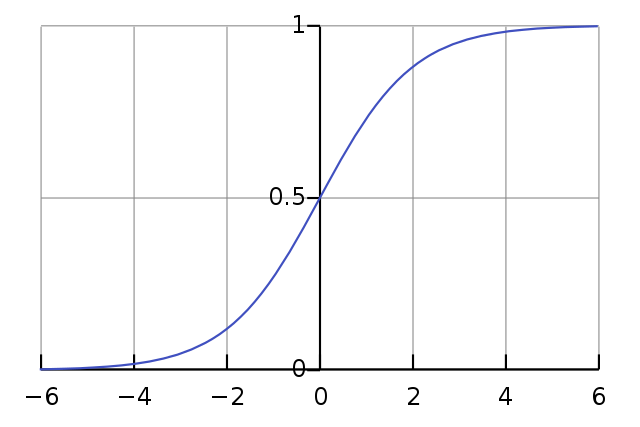
\includegraphics[scale=0.28]{logistic.png}
\end{center}
\item Each parameter is expressed as $\Pi_j=\sigma(a_j)$
and the $a_j$s are used as the parameters
\item Using the chain rule of derivatives
$$\frac{\partial P(e_t)}{\partial a_j}=\sigma(a_j)\cdot(1-\sigma(a_j))\frac{\partial P(f(\vecranvar{X}))}{\partial \Pi_j}$$
\end{itemize}
\end{frame}


\begin{frame}
 \frametitle{ProbLog2}

\begin{itemize}
\item
ProbLog2 includes 
LFI-ProbLog\index{LFI-ProbLog} [Gutmann et al PKDD 2011]   that learns the parameters of ProbLog programs from partial interpretations.
\item Partial interpretations specify the truth value of some but not
necessarily all ground atoms.
\item  $\cI=\pair{I_T}{I_F}$: the atoms
in $I_T$ are true and those in $I_F$ are false.
\item $\cI=\pair{I_T}{I_F}$  can be associated with a conjunction $q(\cI)=\bigwedge_{a\in I_T}\wedge\bigwedge_{a\in I_F}\lpnot a$.
\end{itemize}
\end{frame}
\begin{frame}
 \frametitle{LFI-ProbLog}
\begin{definition}[LFI-ProbLog learning problem]
\index{ProbLog2!parameter learning problem}
Given a ProbLog program \defpprog with unknown parameters and a set $E=\{\cI_1,\ldots,\cI_T\}$ of partial interpretations (the examples), find the value of the  parameters $\boldsymbol{\Pi}$ of \defpprog that maximize the 
likelihood of the examples, i.e., solve
$$\argmax_{\boldsymbol{\Pi}}P(E)=\argmax_{\boldsymbol{\Pi}}\prod_{t=1}^T P(q(\cI_t))$$
\end{definition}
\end{frame}
\begin{frame}
 \frametitle{LFI-ProbLog}
 \begin{itemize}
 \item EM algorithm 
 \item A d-DNNF circuit for each partial interpretation $\cI=\pair{I_T}{I_F}$
by using the ProbLog2 algorithm inference algorithm with the evidence $q(\cI)$.
\item
A Boolean random variable $X_{ij}$  is associated with each ground probabilistic fact $f_i\theta_j$. 
\item For each example $\cI$,  variable $X_ {ij}$ and $x\in\{0,1\}$, LFI-ProbLog  computes
$P(X_{ij}=x|\cI)$. 
\item 
LFI-ProbLog computes $P(X_{ij}=x|\cI)$ by computing $P(X_{ij}=x,\cI)$ using  
 Procedure \textsc{CircP} 
\end{itemize}
\end{frame}
\begin{frame}
 \frametitle{Example of a d-DNNF Circuit}
 \begin{center}
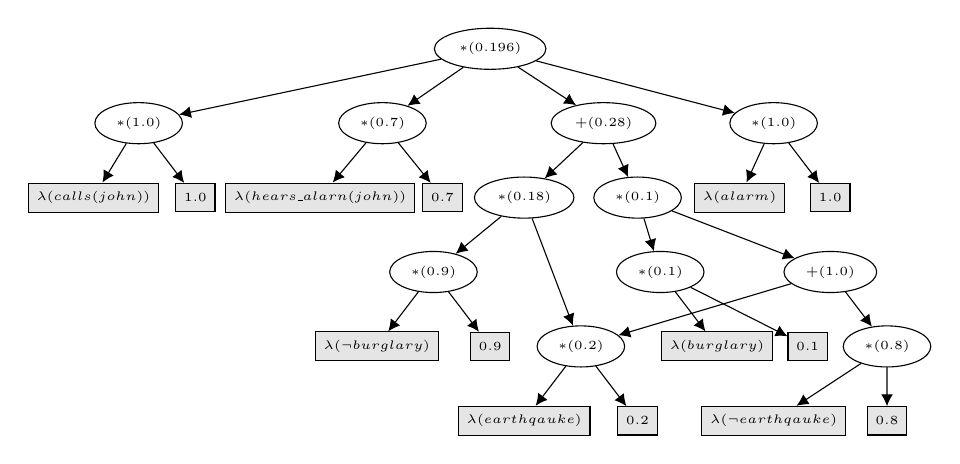
\begin{tikzpicture}
[scale=0.9, transform shape,every node/.style={font=\tiny},x=1.6cm,y=0.7cm,
zeroarrow/.style = {-{Latex[length=1.5mm,width=1.5mm]},dashed},
  onearrow/.style = {-{Latex[length=1.5mm,width=1.5mm]},solid},
  c/.style = {ellipse,draw,solid},
  r/.style = {rectangle,draw,solid,fill=black!10!white},minimum height=4mm]
%[place/.style={shape=ellipse}]
%,draw=blue!50,fill=blue!20,thick,inner sep=0pt,minimum size=6mm},

\node[c] (root) at (0,0) {$*(0.196)$};
   \node[c] (callsj) at (-3.1,-1.5) {$*(1.0)$};
      \node[r] (callsjl) at (-3.5,-3) {$\lambda(calls(john))$};
      \node[r] (callsjw) at (-2.6,-3) {$1.0$};

\node[c] (h) at (-0.95,-1.5) {$*(0.7)$};
\node[r] (hl) at (-1.5,-3) {$\lambda(hears\_alarn(john))$};
\node[r] (hw) at (-0.42,-3) {$0.7$};

\node[c] (al) at (2.5,-1.5) {$*(1.0)$};
\node[r] (all) at (2.2,-3) {$\lambda(alarm)$};
\node[r] (alw) at (3,-3) {$1.0$};
\node[c] (vee1) at (1,-1.5) {$+(0.28)$};
\node[c] (wedge1) at (0.3,-3) {$*(0.18)$};
\node[c] (wedge2) at (1.3,-3) {$*(0.1)$};

      \node[c] (nb) at (-0.5,-4.5) {$*(0.9)$};
      \node[r] (nbl) at (-1,-6) {$\lambda(\neg burglary)$};
      \node[r] (nbw) at (-0,-6) {$0.9$};
      \node[c] (vee2) at (3,-4.5) {$+(1.0)$};
   \node[c] (e) at (0.8,-6) {$*(0.2)$};
   \node[r] (el) at (0.3,-7.5) {$\lambda(earthqauke)$};
   \node[r] (ew) at (1.3,-7.5) {$0.2$};
         \node[c] (b) at (1.5,-4.5) {$*(0.1)$};
         \node[r] (bl) at (2,-6) {$ \lambda(burglary)$};
         \node[r] (bw) at (2.8,-6) {$0.1$};
   \node[c] (ne) at (3.5,-6) {$*(0.8)$};
   \node[r] (nel) at (2.5,-7.5) {$\lambda(\neg earthqauke)$};
   \node[r] (new) at (3.5,-7.5) {$0.8$};

\path[onearrow] (root) edge (callsj);
\path[onearrow] (callsj) edge (callsjl);
\path[onearrow] (callsj) edge (callsjw);
\path[onearrow] (root) edge (h);
\path[onearrow] (h) edge (hl);
\path[onearrow] (h) edge (hw);
\path[onearrow] (root) edge (vee1);
\path[onearrow] (root) edge (al);
\path[onearrow] (al) edge (all);
\path[onearrow] (al) edge (alw);
\path[onearrow] (vee1) edge (wedge1);
\path[onearrow] (vee1) edge (wedge2);
\path[onearrow] (wedge1) edge (nb);
\path[onearrow] (nb) edge (nbl);
\path[onearrow] (nb) edge (nbw);
\path[onearrow] (wedge1) edge (e);
\path[onearrow] (e) edge (el);
\path[onearrow] (e) edge (ew);
\path[onearrow] (wedge2) edge (b);
\path[onearrow] (b) edge (bl);
\path[onearrow] (b) edge (bw);
\path[onearrow] (wedge2) edge (vee2);
\path[onearrow] (vee2) edge (e);
\path[onearrow] (vee2) edge (ne);
\path[onearrow] (ne) edge (nel);
\path[onearrow] (ne) edge (new);

\end{tikzpicture}
\end{center}
\end{frame}

\begin{frame}
 \frametitle{Computing Expectations}
$$\WMC(\phi)=\sum_{\omega\in SAT(\phi)}\prod_{l\in \omega}w(l)\lambda(l)=\sum_{\omega\in SAT(\phi)}\prod_{l\in \omega}w(l)\prod_{l\in \omega}\lambda(l)$$
\begin{itemize}
\item
We want to compute 
$P(q|e)$ for all atoms $q\in Q$. 
\item Partial derivative $\frac{\partial f}{\partial \lambda_q}$ for an atom $q$:\index{partial derivative}
\begin{eqnarray*}
\frac{\partial f}{\partial \lambda_q}&=&\sum_{\omega\in SAT(\phi),q\in\omega}\prod_{l\in \omega}w(l)\prod_{l\in \omega,l\neq q}\lambda(l)=\\
&&\sum_{\omega\in SAT(\phi),q\in\omega}\prod_{l\in \omega}w(l)=\\
&&P(e,q)
\end{eqnarray*}
\item If we compute the partial derivatives of $f$ for all indicator variables $\lambda_q$,  we get $P(q,e)$ for all atoms $q$.
\end{itemize}
\end{frame}
\begin{frame}
 \frametitle{Computing Expectations}
 \begin{itemize}
\item  $v(n)$: valueof each
node $n$ 
\item 
$d(n)=\frac{\partial v(r)}{\partial v(n)}$.
\item $d(r)=1$ 
\item By the chain rule of calculus, for an
arbitrary non-root node $n$ with  $p$ indicating its parents
$$d(n)=\sum_{p}\frac{\partial v(r)}{\partial v(p)}\frac{\partial v(p)}{\partial v(n)}=\sum_{p}d(p)\frac{\partial v(p)}{\partial v(n)}.$$
\end{itemize}
\end{frame}
\begin{frame}
 \frametitle{Computing Expectations}
 \begin{itemize}
\item 
If  $p$ is a multiplication node with $n'$ indicating its children
$$\frac{\partial v(p)}{\partial v(n)}=\frac{\partial v(n)\prod_{n'\neq n} v(n')}{\partial v(n)}=\prod_{n'\neq n} v(n').$$
\item 
If parent $p$ is an addition node with $n'$ indicating its children
$$\frac{\partial v(p)}{\partial v(n)}=\frac{\partial v(n)+\sum_{n'\neq n} v(n')}{\partial v(n)}=1.$$
\item  $+p$ an addition parent of $n$ and  $*p$ a multiplication parent of $n$:
$$d(n)=\sum_{+p}d(+p)+\sum_{*p}d(*p)\prod_{n'\neq n} v(n').$$
\item
If $v(n)\neq 0$. 
 $$d(n)=\sum_{+p}d(+p)+\sum_{*p}d(*p)v(*p)/v(n).$$
\end{itemize}
\end{frame}


\begin{frame}
 \frametitle{CircP}
% The d-DNNF circuit is visited twice, once bottom up to compute $P(q(\cI))$ and
%once top down to compute $P(X_{ij}=x|\cI)$ for all the variables $X_{ij}$ and values $x$. 
  \begin{scriptsize}
\begin{algorithmic}[1]
\Procedure{CircP}{$circuit$}
\State assign values to leaves
\ForAll{non-leaf node $n$ with children $c$ (visit children before parents)}
  \If{$n$ is an addition node}
    \State $v(n)\gets \sum_{c}v(c)$
  \Else
    \State $v(n)\gets \prod_{c}v(c)$
  \EndIf
\EndFor
\State $d(r)\gets 1$, $d(n)=0$ for all non-root nodes
\ForAll{non-root node $n$ (visit  parents before children)}
  \ForAll{parents $p$ of $n$}
    \If{$p$ is an addition parent}
      \State $d(n)=d(n)+d(p)$
    \Else
      \State $d(n)\gets d(n)+d(p)v(p)/v(n)$
    \EndIf
  \EndFor
\EndFor
\EndProcedure
\end{algorithmic}
  \end{scriptsize}
\end{frame}
%
%\begin{frame}[fragile]
%  \frametitle{Input File}
%Preamble
%\begin{small}
%\begin{verbatim}
%:-use_module(library(slipcover)).
%:- if(current_predicate(use_rendering/1)).
%:- use_rendering(c3).
%:- use_rendering(lpad).
%:- endif.
%:-sc.
%:- set_sc(random_restarts_number,10).
%:- set_sc(seed,seed(3020)).
%:- set_sc(epsilon_em,0.001).
%:- set_sc(epsilon_em_fraction,0.001).
%:- set_sc(verbosity,1).
%\end{verbatim}
%\end{small}
%See \url{http://cplint.eu/help/help-cplint.html} for a list of options
%
%\end{frame}
%
%
%\begin{frame}[fragile]
%  \frametitle{Input File}
%Theory for parameter learning and background
%\begin{small}
%\begin{verbatim}
%bg([]).
%in([
%(pos:0.5 :-
% 	circle(A),
% 	in(B,A)),
%(pos:0.5 :-
% 	circle(A),
% 	triangle(B))]).
%\end{verbatim}
%\end{small}
%
%\end{frame}
%
%
%\begin{frame}[fragile]
%  \frametitle{Input File}
%Data: two formats, models
%\begin{scriptsize}
%\begin{verbatim}
%begin(model(2)).
%pos.
%triangle(o5).
%config(o5,up).
%square(o4).
%in(o4,o5).
%circle(o3).
%triangle(o2).
%config(o2,up).
%in(o2,o3).
%triangle(o1).
%config(o1,up).
%end(model(2)).
%
%begin(model(3)).
%neg(pos).
%circle(o4).
%circle(o3).
%in(o3,o4).
%....
%\end{verbatim}
%\end{scriptsize}
%
%\end{frame}
%
%\begin{frame}[fragile]
%  \frametitle{Input File}
%Data: two formats, keys (internal representation)
%\begin{scriptsize}
%\begin{verbatim}
%pos(2).
%triangle(2,o5).
%config(2,o5,up).
%square(2,o4).
%in(2,o4,o5).
%circle(2,o3).
%triangle(2,o2).
%config(2,o2,up).
%in(2,o2,o3).
%triangle(2,o1).
%config(2,o1,up).
%
%neg(pos(3)).
%circle(3,o4).
%circle(3,o3).
%in(3,o3,o4).
%square(3,o2).
%circle(3,o1).
%in(3,o1,o2).
%....
%\end{verbatim}
%\end{scriptsize}
%
%\end{frame}
%
%\begin{frame}[fragile]
%  \frametitle{Input File}
%\begin{itemize}
%\item
%Folds (a group of examples)
%\item Target predicates \verb|output(<predicate>)|
%\end{itemize}
%\begin{small}
%\begin{verbatim}
%fold(train,[2,3,5,...]).
%fold(test,[490,491,494,...]).
%output(pos/0).
%\end{verbatim}
%\end{small}
%
%\end{frame}
%
%
%\begin{frame}[fragile]
%  \frametitle{Command}
%
%\begin{verbatim}
%induce_par([train],P),
%  test(P,[test],LL,AUCROC,ROC,AUCPR,PR).
%\end{verbatim}
%\url{http://cplint.eu/e/bongard.pl}
%\end{frame}
%
%\begin{frame}
%	\frametitle{EM Algorithm}
%
%\begin{itemize}
%	\item \textit{\myalert{Expectation step}} \ (synthesis)
%
%					\begin{enumerate}
%
%
%
%						\item Expectations $\mathbf{E}[c_{ik0}]$ and $\mathbf{E}[c_{ik1}]$ where $c_{ikx}$ is the number of times a Boolean variable $X_{ijk}$ takes value $x$ for all $C_i$s, $k=1,\ldots,n_i-1$
%$$\mathbf{E}[c_{ikx}]=\sum_{Q}\mathbf{E}[c_{ikx}|Q]$$
%
%\item  Expected counts per query
%						$\mathbf{E}[c_{ikx}|Q]$,
% for all  queries $Q$  and $x\in \{0,1\}$.
% $$\mathbf{E}[c_{ikx}|Q]=\sum_{j\in g(i)}P(X_{ijk}=x|Q)$$
%$ g(i):=\{j|\theta_j$  is  a  substitution  grounding $C_i\}$
%					\end{enumerate}
%
%	\item \textit{\myalert{Maximization step}}
%					  \begin{itemize}
%							\item Updates parameters \myalert{$\pi_{ik}$ representing $P(X_{ijk}=1)$} % for all rules $C_i$ and all groundings $j$
%							\item \textbf{$\pi_{ik}$ = $E[c_{ik\myalert{1}}]$ / ($E[c_{ik0}]$ + $E[c_{ik1}]$)}
%							%\item
%					  \end{itemize}
%\end{itemize}
%
%\end{frame}
%
%\begin{frame}
% \frametitle{Expectation Computation}
%%\begin{itemize}
%%\item {\small \myalert{Complete BDD}: every path contains a node for every level}
%%\end{itemize}
%%{\scriptsize
%%$$
%%\xymatrix@=2.5mm
%%{ X_{111} & &*=<25pt,10pt>[F-:<3pt>]{n_1}
%%\ar@/_/@{-}[ld] \ar@/^/@{--}[dr]\\
%%X_{121}  & *=<25pt,10pt>[F-:<3pt>]{n'_2}\ar@/_/@{-}[d]  \ar@/^/@{--}[d] &&*=<25pt,10pt>[F-:<3pt>]{n_2}
%%\ar@/_/@{-}[dll]\ar@{--}[d]
%%\\
%%X_{211}& *=<25pt,10pt>[F-:<3pt>]{n_3}
%%\ar@{-}[d] \ar@/^/@{--}[drr]  &&*=<25pt,10pt>[F-:<3pt>]{n'_3}
%%\ar@/_/@{-}[d] \ar@/^/@{--}[d]  \\
%%&*=<25pt,10pt>[F]{1} &&*=<25pt,10pt>[F]{0}}
%%$$}
%\begin{itemize}
%\item $P(X_{ijk}=x|Q)=\frac{P(X_{ijk}=x,Q)}{P(Q)}$
%\item  $P(X_{ijk}=x,Q)=\sum_{n\in N(Q),v(n)=X_{ijk}}F(n)B(child_x(n))\pi_{ikx}=\sum_{n\in N(Q),v(n)=X_{ijk}}e^x(n)$
%				\begin{itemize}
%				%\begin{small}
%				\item $\pi_{ikx}$ is $\pi_{ik}$ if $x=1$ and  $(1-\pi_{ik})$ if $x=0$
%				\item $F(n)$ is the \myalert{forward probability}, the probability mass of the paths from the root to $n$
%				\item $B(n)$ is the \myalert{backward probability}, the probability mass of paths from $n$ to the 1-leaf
%				\item $F(n)$ and $B(n)$ are computed by two traversal of the BDD of $Q$
%				\item $e^x(n)$ is the probability mass of paths from the root to the 1 leaf passing through the $x$ branch of $n$
%			%	\end{small}
%				\end{itemize}
%\end{itemize}
%%\begin{itemize}
%%\item {\small If the BDD is not complete deleted paths have to be counted}
%%\end{itemize}
%\end{frame}
%
%



\end{document}


